\section{Limitations}

\paragraph{Not a FluSight leaderboard claim.}
The frozen benchmark is a retrospective FluSurv-NET-style hospitalization-rate
forecasting study. It should not be described as a FluSight challenge result,
a real-time prospective forecast, or evidence of state-of-the-art performance
against operational forecasting systems.

\paragraph{No FluSight, Flusion, or SINDy comparison in this phase.}
The discovery-ablation freeze intentionally focuses on standard forecasting
baselines, hand-specified epidemic baselines, and same-grammar discovery
ablations. It does not include FluSight models, Flusion-style systems, SINDy,
symbolic regression, or other external forecasting frameworks. Those would be
separate comparison projects and should not be implied by the current results.

\paragraph{Grammar and budget dependence.}
Discovery results depend on the bounded grammar, candidate evaluator, scoring
policy, optimizer budget, and candidate-search budget used in
\texttt{configs/discovery\_ablation.yaml}. Exhaustive search covers the current
valid grammar universe, but the grammar itself remains intentionally small.
Random search uses an explicit budget and seed. Conclusions should therefore
be framed as evidence about this controlled discovery space rather than about
all possible epidemic model structures.

\begin{figure}[H]
\centering
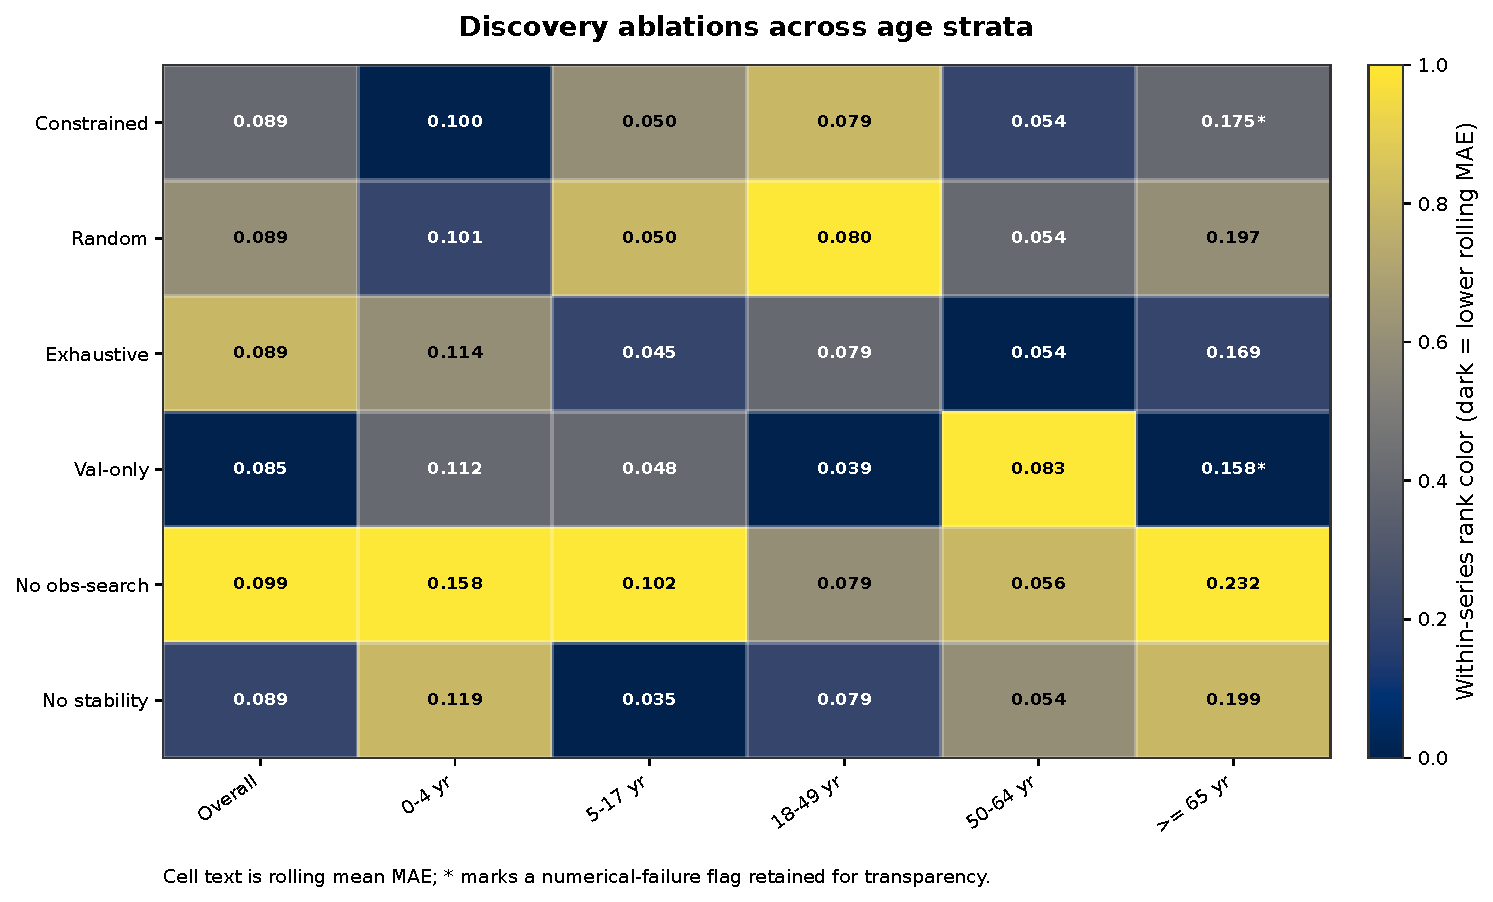
\includegraphics[width=\textwidth]{figures/fig3_discovery_ablation_matrix.pdf}
\caption{Supplementary discovery-ablation matrix. Cell values show
rolling-origin MAE for same-grammar discovery variants, ranked within each age
stratum by color. The figure is diagnostic evidence about the frozen grammar
and budget, not a single-global-winner claim. Flagged
cells are retained for transparency.}
\label{fig:discovery-ablation-matrix}
\end{figure}

\paragraph{Objective dependence.}
Held-out test MAE and rolling-origin MAE do not always select the same model.
The results are best interpreted through objective-aware recommendations:
users prioritizing fixed-split accuracy may choose different models than users
prioritizing rolling-origin stability.

\paragraph{Numerical failure transparency.}
The benchmark retains rows with \texttt{numerical\_failure\_flag=True} in the
artifact tables so that optimizer and prediction-scale issues remain visible.
These flagged rows are not removed from descriptive summaries, but they are
not used to support positive claims. In particular, any statement involving a
flagged model-series row should be treated as descriptive and caveated.

\paragraph{Multi-season robustness is mixed.}
A compact season-separated robustness appendix evaluates completed FluSurv-NET
seasons as independent within-season trajectories. This appendix does not test
previous-season-to-future-season transfer forecasting and uses a reduced
budget. Its pediatric results are mixed across seasons, so we treat the frozen
discovery-ablation benchmark as the clearest evidence for the \texttt{0-4 yr}
delayed-observation finding and use the multi-season check as a robustness
caveat rather than as a stronger global claim.

\paragraph{Offline policy layer is not an autonomous scientific agent.}
The verifier and selection-policy layer is deterministic, offline, and
restricted to compact summary CSVs. It is not an autonomous scientific agent,
does not run new model fits, and should not be read as a replacement for
prospective experiments. Budgeted replay uses frozen compact rows. The
optional API-assisted proposal smoke test is constrained to structured JSON
from an explicit allowlist; API output is verifier-gated, cannot generate
model code, and is used only to evaluate proposal validity and diversity. The
toy observation-label recovery task is generic numerical validation only; it
is a software check for policy logic rather than evidence of real-world
mechanism discovery.

\paragraph{Candidate execution replay is budget-efficiency evidence only.}
The Stage 6 candidate-execution evaluation supports proposal ordering and
candidate-budget efficiency claims only. Its synthetic layer uses generic toy
time-series tasks. Its real-data layer is frozen replay over compact summary
rows and does not perform new forecasting experiments or real-data model
refitting. Test metrics in the replay tables are post-hoc descriptive only.
The API path is disabled in the committed Stage 6 evaluation, so real API
evidence remains limited to proposal-quality smoke testing. These results
should not be described as improved forecasting performance, autonomous
science, or real-world mechanism recovery.

\paragraph{Bounded real candidate execution is not an operational benchmark.}
The Stage 7 bounded execution evaluation uses reduced fitting and search
budgets, a small set of selected series, and an explicit allowlist of
repository models. It is useful for testing whether verifier-gated proposal
ordering reaches good candidates under fixed budgets, but it is not a
prospective or operational forecasting benchmark. Real API access is disabled
in the committed Stage 7 evaluation; the \texttt{mock\_api\_proposer} is a
structured stand-in, while real API evidence remains limited to the earlier
proposal-quality smoke test. These results do not imply API autonomy, real
mechanism discovery, FluSight leaderboard performance, or state-of-the-art
forecasting performance.

\paragraph{Cross-provider proposer results depend on adapters and schemas.}
The Stage 9 cross-provider benchmark evaluates OpenAI, Claude, Gemini, and
DeepSeek as constrained structured proposers, not as forecasting systems,
clinical decision providers, or autonomous scientific agents. Results depend
on provider adapters, structured-output schemas, token budgets, prompt
compaction, and API behavior at the time of the run. Gemini required
provider-native structured-output integration and compact schema-guided
prompting before entering the same verifier-gated comparison. The reported
metrics support proposal-quality and frozen-replay budget-efficiency
comparisons only; they do not imply provider superiority for forecasting,
medical recommendations, FluSight performance, real-world mechanism recovery,
or state-of-the-art results. Iterative feedback is also not automatically
better than single-shot proposal under a small explicit allowlist.

\paragraph{Synthetic structured recovery is software validation.}
The final expanded structured recovery sweep uses generic toy time series with
known direct, lagged, mixture, and proxy observation labels. These tasks help
test whether deterministic selection policies can recover labels under a
controlled setup, but they do not use real FluSurv-NET data, do not prove
recovery of real-world epidemic mechanisms, and should not be interpreted as
new real-data forecasting evidence. The API-assisted proposal path is disabled
in this sweep.

\begin{figure}[H]
\centering
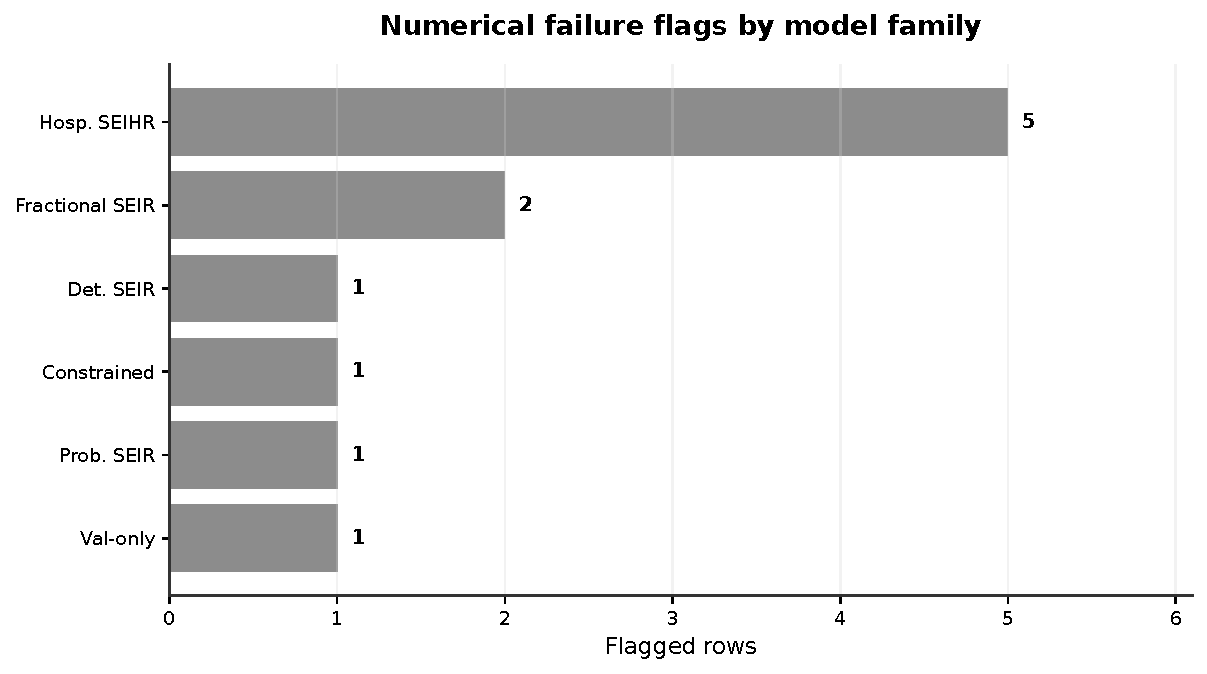
\includegraphics[width=0.88\textwidth]{figures/fig5_numerical_failure_audit.pdf}
\caption{Numerical failure flags by model family. Flagged rows are retained in
the frozen artifacts for transparency and are not used to support positive
claims.}
\label{fig:numerical-failure-audit}
\end{figure}

\paragraph{Retrospective, dataset-specific evidence.}
The strongest positive result is concentrated in the pediatric
\texttt{0-4 yr} series. Adult strata often favor simpler forecasting baselines
or manual epidemic models. The paper should therefore avoid claiming global
discovery dominance and instead emphasize when observation-aware discovery is
useful, when simpler models suffice, and why age-aware model selection is
necessary.
